\documentclass[11pt,a4paper]{article}


\usepackage[utf8]{inputenc}
\usepackage[T1]{fontenc}
\usepackage[polish,english]{babel}
\usepackage[a4paper,margin=2.5cm]{geometry}
\usepackage{setspace}
\usepackage{amsmath,amssymb,amsfonts}
\usepackage{graphicx}
\usepackage{booktabs}
\usepackage{multirow}
\usepackage{array}
\usepackage{float}
\usepackage[hidelinks]{hyperref}
\usepackage{xcolor}
\usepackage{caption}
\usepackage{subcaption}
\usepackage{enumitem}
\usepackage{csquotes}
\usepackage{listings}
\usepackage{fancyhdr}
\usepackage{titlesec}
\usepackage{authblk}


\onehalfspacing
\setlength{\parindent}{0pt}
\setlength{\parskip}{0.6em}

\hypersetup{
    colorlinks=true,
    linkcolor=blue,
    citecolor=blue,
    urlcolor=blue,
    pdftitle={Raport projektowy},
    pdfauthor={Jakub Jurzak, Marcin Osojca}
}

\pagestyle{fancy}
\fancyhf{}
\rhead{Eksploracja i wizualizacja danych}
\lhead{Raport projektowy}
\cfoot{\thepage}

\titleformat{\section}{\large\bfseries}{\thesection.}{0.5em}{}
\titleformat{\subsection}{\normalsize\bfseries}{\thesubsection.}{0.5em}{}

\graphicspath{{output/}}


\title{\textbf{Automatyczne wykrywanie liczby klastrów w danych}\\
\large Porównanie metod Elbow, Silhouette oraz Gap Statistic}

\author[1]{Jakub Jurzak}
\author[1]{Marcin Osojca}
\affil[1]{Informatyka mgr. dzienne 3 sem. / Eksploracja i Wizualizacja Danych}
\date{\today}


\begin{document}

\selectlanguage{polish}

\maketitle

\begin{abstract}
Celem pracy było zbadanie problemu oceny skuteczności i wiarygodności popularnych heurystyk w określaniu optymalnej liczby klastrów. 
Przeprowadzono analizę wielowymiarowego zbioru danych \textit{Dry Bean Dataset}, wykonano preprocessing (standaryzację i redukcję wymiarowości PCA), eksploracyjną analizę danych oraz porównano wybrane metody wyznaczania liczby klastrów (Elbow Method, Silhouette Score, Gap Statistic). Oceniono ich skuteczność przy użyciu metryk Adjusted Rand Index (ARI) oraz Normalized Mutual Information (NMI) na tle rzeczywistych etykiet (ground truth = 7 klas).
Uzyskane wyniki wskazują, że żadna z analizowanych metod nie wskazała poprawnie liczby klastrów $k=7$ ze względu na silne nakładanie się klas, przy czym Gap Statistic okazała się najskuteczniejsza, sugerując $k=5$.
\end{abstract}

\textbf{Słowa kluczowe:} eksploracja danych, wizualizacja danych, uczenie maszynowe, klasteryzacja, ocena liczby klastrów, Dry Bean Dataset

\section{Wprowadzenie}

Eksploracja danych stanowi istotny element współczesnej analizy danych, łącząc metody statystyczne, uczenie maszynowe oraz narzędzia wizualizacyjne. 
W praktyce celem analizy nie jest jedynie budowa modelu, ale również zrozumienie struktury danych, identyfikacja zależności oraz interpretacja wyników.

Celem niniejszego projektu jest:
\begin{itemize}[leftmargin=1.5cm]
    \item sformułowanie problemu badawczego dotyczącego wykrywania liczby klastrów,
    \item przygotowanie i eksploracja danych wielowymiarowych,
    \item porównanie wybranych metod analitycznych (Elbow, Silhouette, Gap Statistic),
    \item ocena jakości wyników na podstawie znanych etykiet klas (ground truth),
    \item interpretacja rezultatów z wykorzystaniem wizualizacji.
\end{itemize}

Główne pytania badawcze:
\begin{enumerate}[leftmargin=1.5cm]
    \item Która z analizowanych miar najdokładniej wskaże rzeczywistą liczbę klas ($k=7$) w zbiorze Dry Bean Dataset?
    \item Jak kształt i stopień nakładania się klastrów wpływają na skuteczność poszczególnych metod oceny?
    \item W jakich scenariuszach miary bazujące na odległościach wewnątrz- i międzygrupowych zawodzą?
\end{enumerate}

\section{Opis danych}

\subsection{Źródło danych}

W projekcie wykorzystano zbiór danych \textit{Dry Bean Dataset}, pochodzący z repozytorium UCI Machine Learning Repository.

\subsection{Charakterystyka zbioru}

Zbiór "Dry Bean Dataset" zawiera informacje o cechach morfologicznych oraz wymiarach wyekstrahowanych z obrazów 7 różnych zarejestrowanych gatunków fasoli. Cechy te charakteryzują się różną wariancją, a niektóre gatunki (klastry) są do siebie bardzo podobne.
W ramach projektu algorytmy grupujące działają w sposób w pełni nienadzorowany, a dostępna etykieta klasy służy jedynie do końcowej oceny metod.

Zbiór danych zawiera:
\begin{itemize}[leftmargin=1.5cm]
    \item liczbę obserwacji: \textbf{13\,611},
    \item liczbę zmiennych: \textbf{17} (16 cech numerycznych + 1 kategoryczna etykieta klasy),
    \item typy zmiennych: \textit{numeryczne (ciągłe), kategoryczna (nominalna)},
    \item braki danych: \textbf{Brak}.
\end{itemize}

\begin{table}[H]
\centering
\caption{Wybrane zmienne z użytego zbioru danych}
\begin{tabular}{lll}
\toprule
\textbf{Zmienna} & \textbf{Typ} & \textbf{Opis} \\
\midrule
Area & numeryczna & Pole powierzchni ziarna fasoli (liczba pikseli) \\
Perimeter & numeryczna & Obwód ziarna fasoli \\
Compactness & numeryczna & Miara zwartości kształtu (proporcja pola do obwodu) \\
Class & kategoryczna & Etykieta gatunku fasoli (używana wyłącznie do walidacji) \\
\bottomrule
\end{tabular}
\end{table}

\section{Metodologia}

\subsection{Przygotowanie danych}

W etapie preprocessingu wykonano następujące operacje:
\begin{itemize}[leftmargin=1.5cm]
    \item usunięcie etykiety klasy (\texttt{Class}) ze zbioru treningowego dla analizy nienadzorowanej,
    \item standaryzację wszystkich cech numerycznych za pomocą \texttt{StandardScaler} (średnia 0, odchylenie standardowe 1), co jest wymagane przez algorytmy bazujące na odległości euklidesowej,
    \item redukcję wymiarowości przy użyciu analizy głównych składowych (PCA). Wybrano liczbę składowych pozwalającą zachować 95\% wariancji oryginalnych danych (4 składowe główne).
\end{itemize}

\subsection{Eksploracyjna analiza danych}

W ramach EDA przeprowadzono:
\begin{itemize}[leftmargin=1.5cm]
    \item analizę liczebności klas w celu zbadania zbalansowania zbioru,
    \item analizę statystyk opisowych wygenerowaną do zewnętrznego pliku raportu,
    \item analizę rozkładów zmiennych morfologicznych przy użyciu histogramów zgrupowanych,
    \item badanie korelacji cech i współzależności z wykorzystaniem macierzy korelacji.
\end{itemize}

\subsection{Zastosowane metody}

W pracy porównano następujące metody oceny optymalnej liczby klastrów oparte na algorytmie KMeans:
\begin{itemize}[leftmargin=1.5cm]
    \item \textbf{Elbow Method (Metoda łokcia):} Polega na obliczeniu sumy kwadratów odległości wewnątrz klastrów (WCSS) dla kolejnych wartości $k$. Punktem łokcia jest $k$, przy którym spadek WCSS ulega zauważalnemu wypłaszczeniu.
    \begin{equation}
        \text{WCSS}(k) = \sum_{i=1}^{k} \sum_{\mathbf{x} \in C_i} \|\mathbf{x} - \boldsymbol{\mu}_i\|^2
    \end{equation}
    
    \item \textbf{Silhouette Score:} Mierzy jakość klasteryzacji na podstawie spójności wewnątrzgrupowej i separacji międzygrupowej. Wynik dąży do 1 dla doskonałych klasteryzacji.
    \begin{equation}
        s(i) = \frac{b(i) - a(i)}{\max\{a(i),\, b(i)\}}
    \end{equation}
    gdzie $a(i)$ to średnia odległość wewnątrz klastra, $b(i)$ to minimalna średnia odległość do najbliższego obcego klastra.
    
    \item \textbf{Gap Statistic (Statystyka luki):} Porównuje WCSS obserwowanych danych z oczekiwaną wartością WCSS dla danych wygenerowanych z rozkładu jednorodnego. Optymalne $k$ to najmniejsza wartość spełniająca kryterium: $\text{Gap}(k) \geq \text{Gap}(k+1) - s_{k+1}$.
    \begin{equation}
        \text{Gap}(k) = E^*[\log W_k] - \log W_k
    \end{equation}
\end{itemize}

\subsection{Metody oceny}

Do końcowej oceny jakości metod wykorzystano miary walidacji zewnętrznej poprzez porównanie uzyskanych klasteryzacji z etykietami ground truth:
\begin{itemize}[leftmargin=1.5cm]
    \item \textbf{Adjusted Rand Index (ARI):} Skorygowany indeks Randa mierzący podobieństwo dwóch grupowań, uwzględniający przypisania losowe. Zakres $[-1, 1]$, gdzie wartości wyższe oznaczają większą zgodność.
    \item \textbf{Normalized Mutual Information (NMI):} Znormalizowana miara informacji wzajemnej, skalowana do zakresu $[0, 1]$.
\end{itemize}

\section{Analiza eksploracyjna danych}

\subsection{Statystyki opisowe i rozkład klas}

Zbiór cechuje się niezbalansowanym rozkładem klas. Jak widać na Rysunku \ref{fig:class_dist}, klasa \textit{Dermason} stanowi największą grupę, podczas gdy klasa \textit{Bombay} występuje znacznie rzadziej. 

\begin{figure}[H]
    \centering
    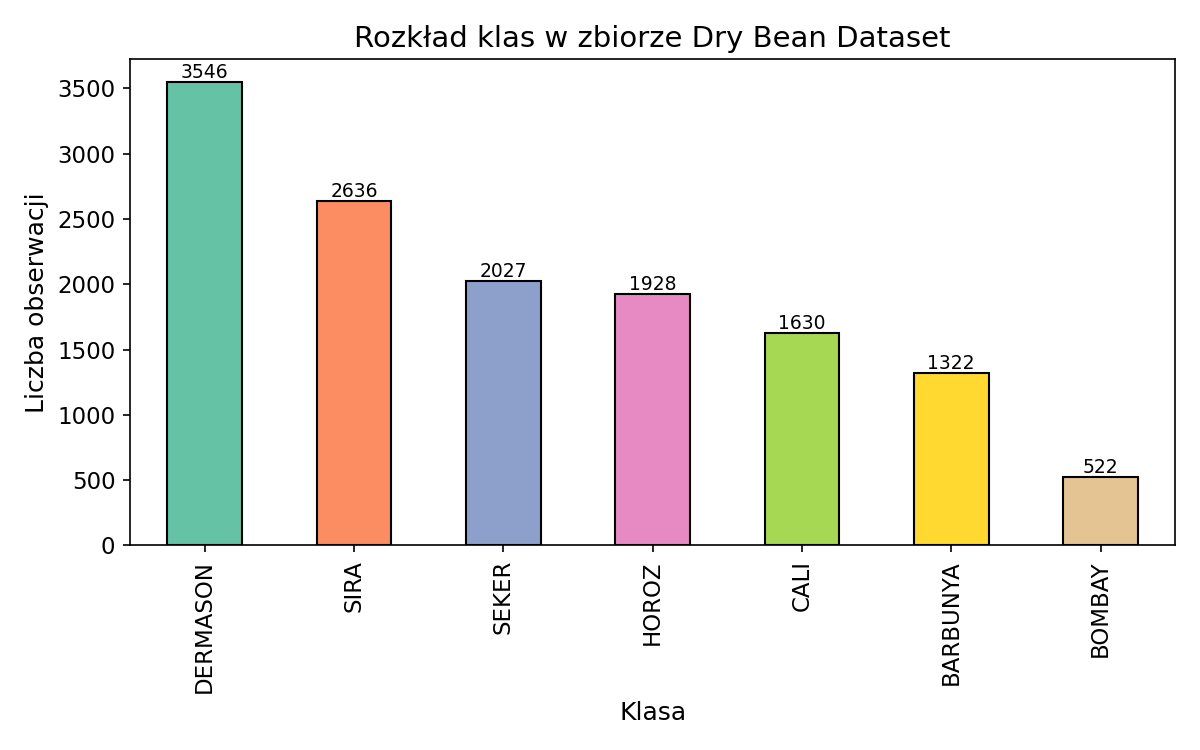
\includegraphics[width=0.65\textwidth]{class_distribution.png}
    \caption{Rozkład liczebności poszczególnych klas w zbiorze danych}
    \label{fig:class_dist}
\end{figure}

\subsection{Analiza zależności}

Większość cech wymiarowych wykazuje bardzo silną korelację dodatnią ($r > 0.9$). Przykładowo wymiary związane bezwzględnie z rozmiarem fasoli (Area, Perimeter, MajorAxisLength, ConvexArea, EquivDiameter) dostarczają redundantnych informacji.

\begin{figure}[H]
    \centering
    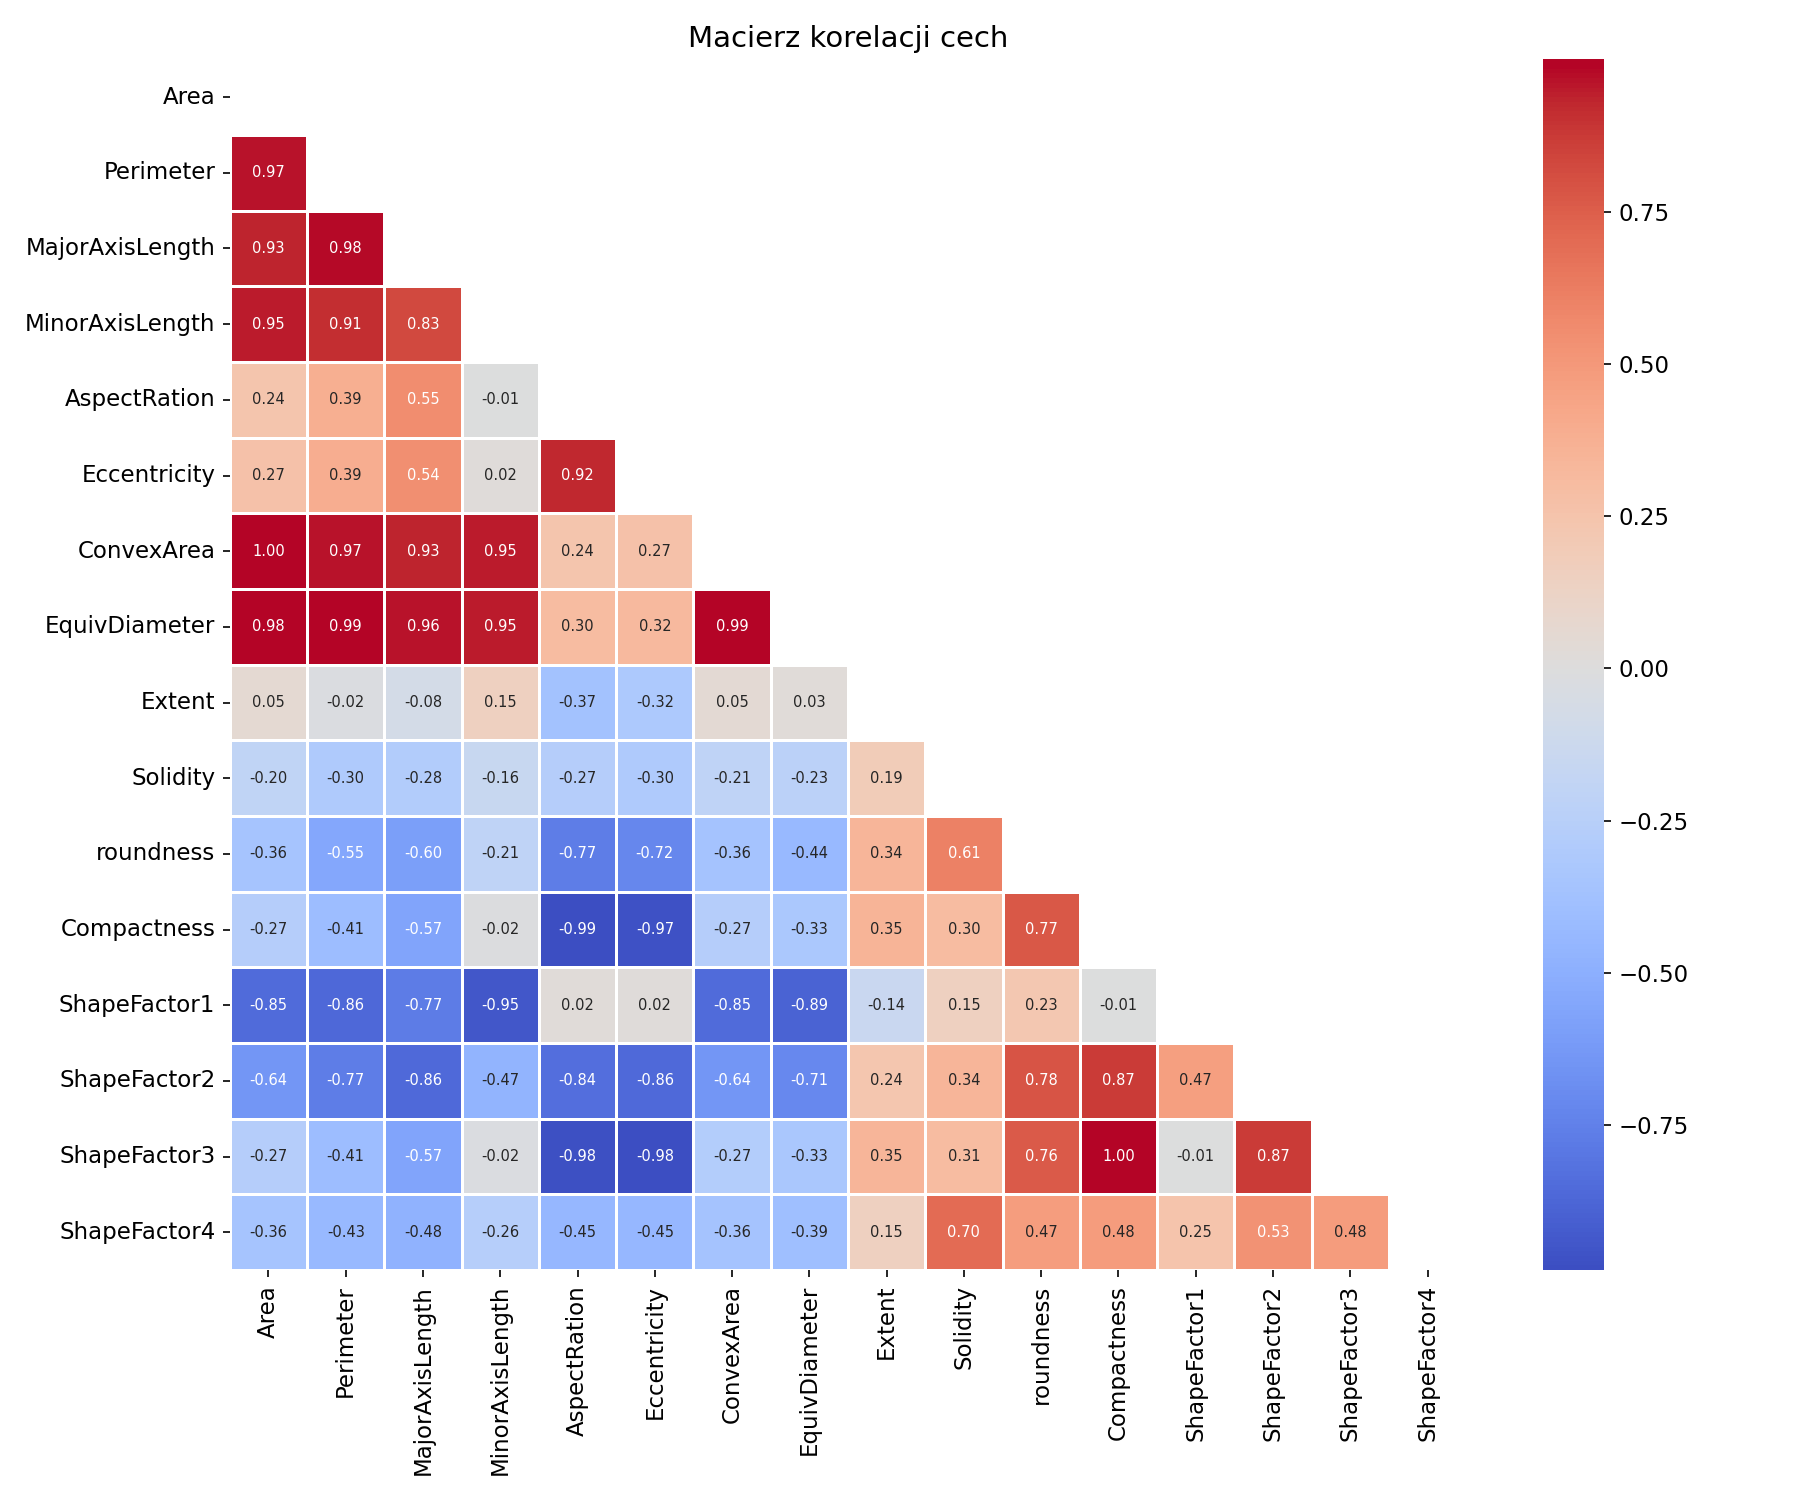
\includegraphics[width=0.75\textwidth]{correlation_heatmap.png}
    \caption{Macierz korelacji dla zmiennych numerycznych}
\end{figure}

\subsection{Wizualizacja rozkładów}

Histogramy wybranych cech ukazują częściowe nakładanie się rozkładów dla poszczególnych klas. Niektóre współczynniki, takie jak Compactness czy Eccentricity, posiadają wielomodalne kształty, co pozwala odróżnić pewne podgrupy gatunków, jednak granice między nimi są rozmyte.

\begin{figure}[H]
    \centering
    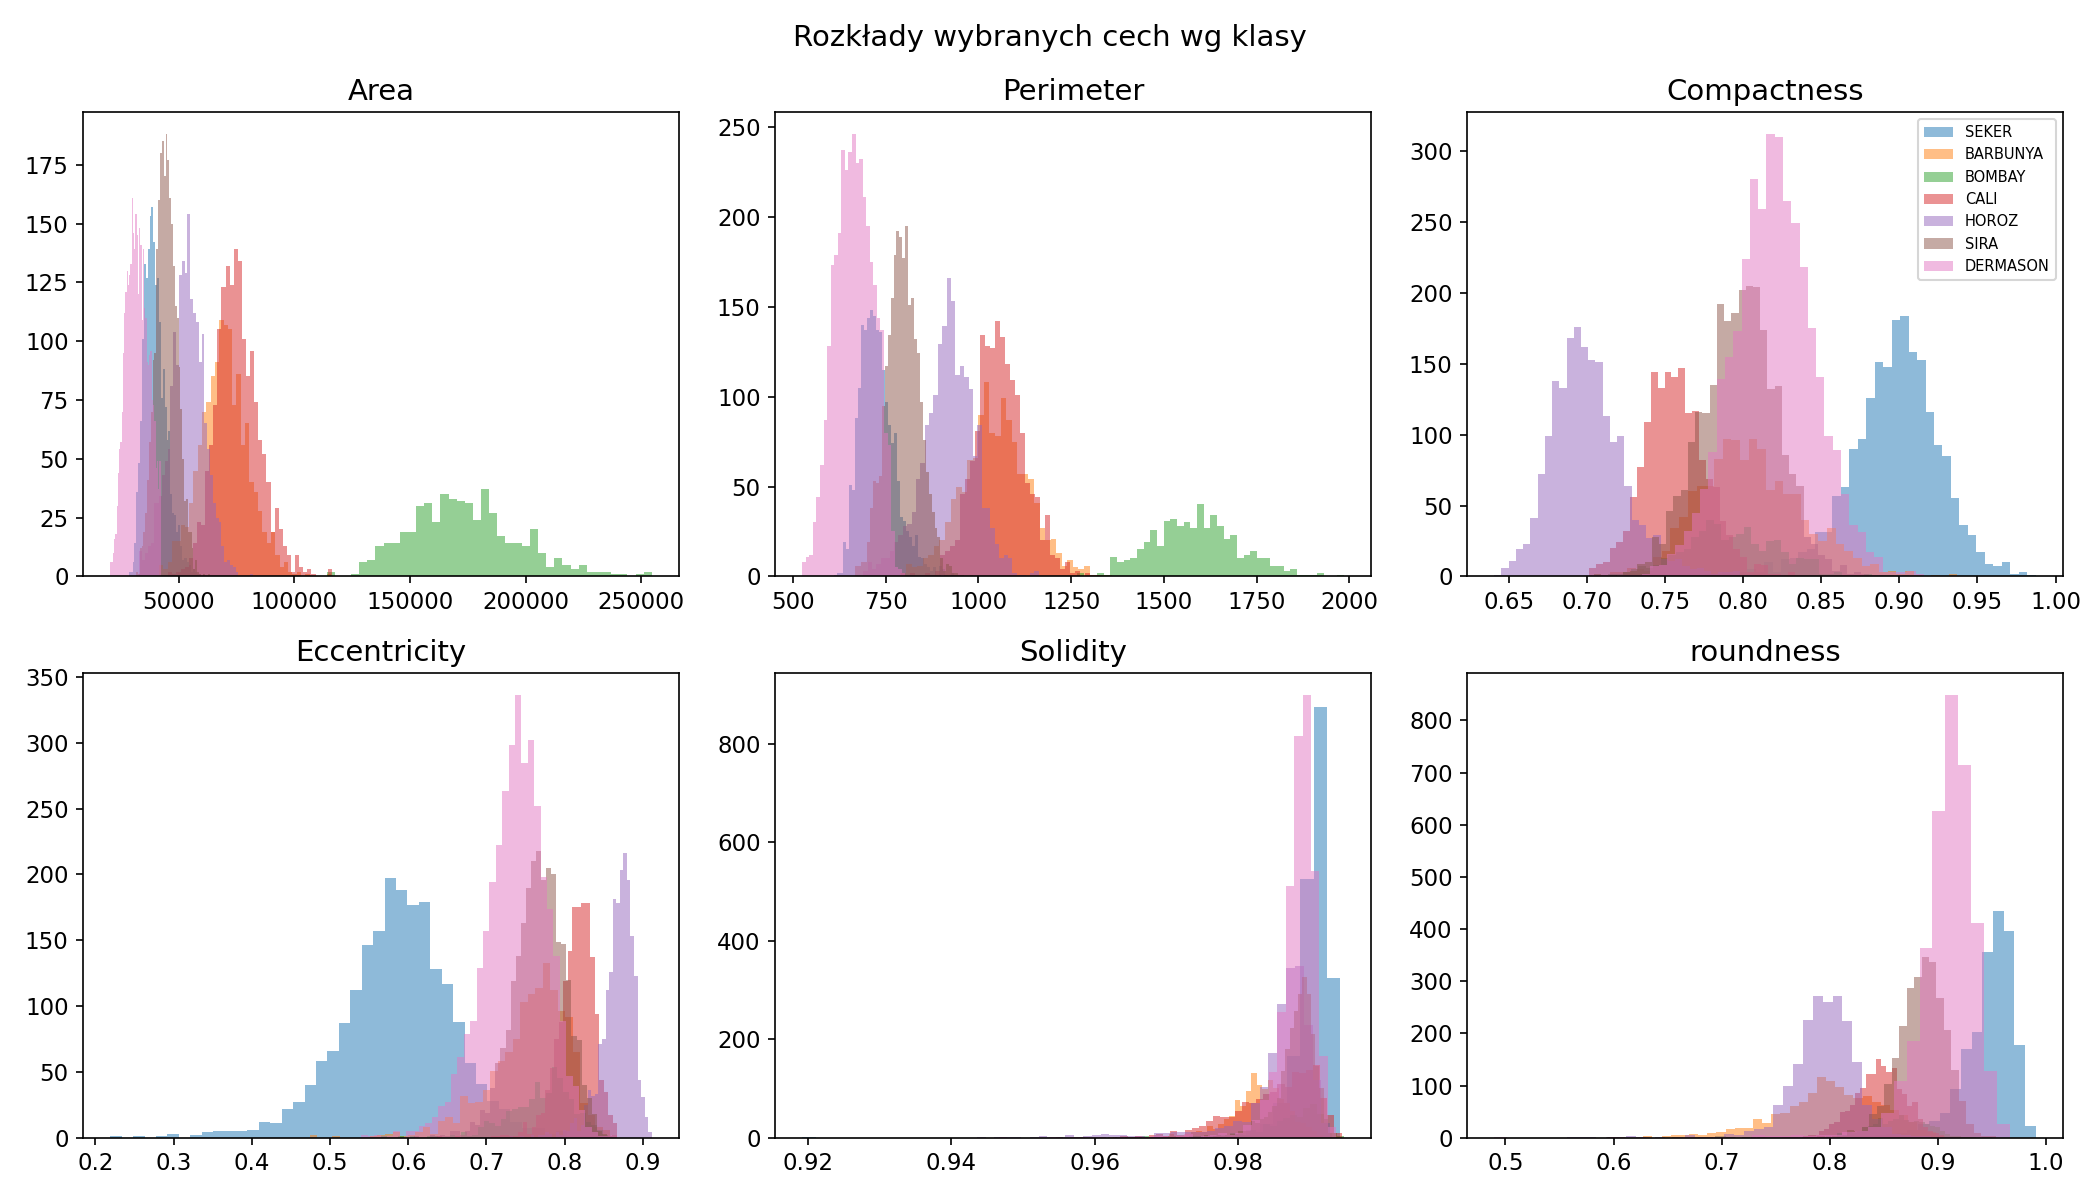
\includegraphics[width=0.8\textwidth]{feature_distributions.png}
    \caption{Histogramy wybranych cech morfologicznych z podziałem na klasy}
\end{figure}

\section{Eksperymenty i wyniki}

\subsection{Konfiguracja eksperymentów}

Klasteryzacja została przeprowadzona w wariancie nienadzorowanym na zbiorze poddanym redukcji PCA (4 składowe główne). Dla każdej metody zbadano liczbę klastrów w przedziale $k \in [2, 15]$. Algorytmem bazowym był KMeans (z inicjalizacją k-means++ i 10 próbami losowymi). 
Wizualizację klastrów przeprowadzono na przestrzeni 2D (2 pierwsze składowe główne PCA), aby zaobserwować strukturę i ewentualne nakładanie się skupisk.

\begin{figure}[H]
    \centering
    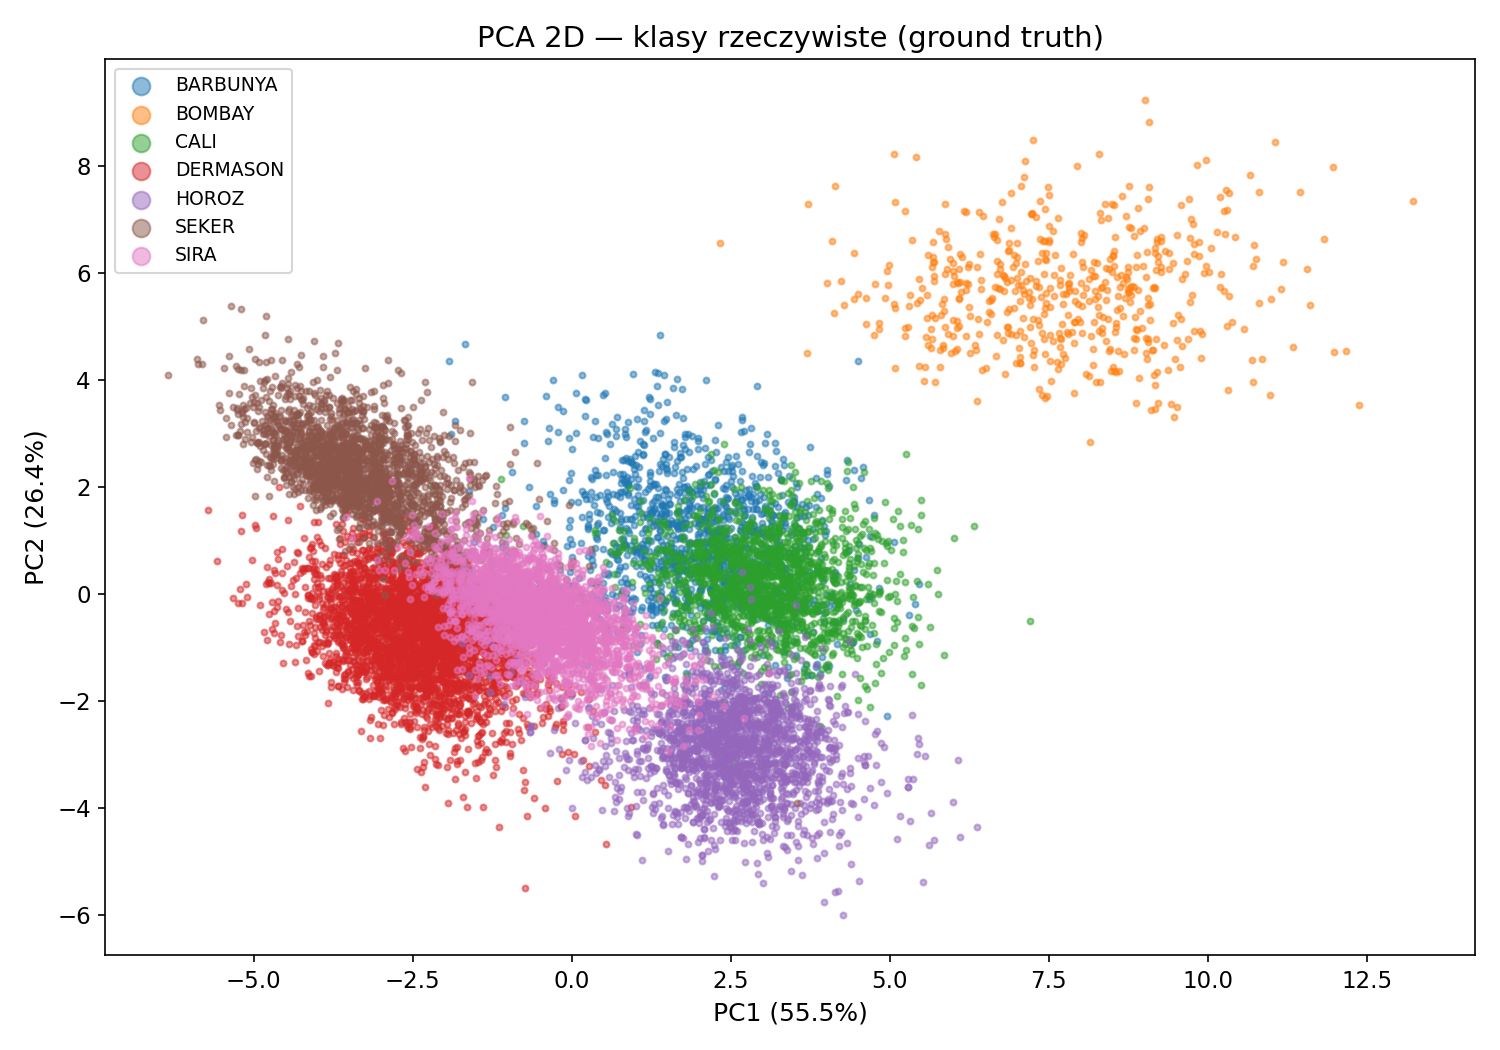
\includegraphics[width=0.65\textwidth]{pca_2d_ground_truth.png}
    \caption{Projekcja PCA 2D z kolorowaniem wg klas rzeczywistych}
\end{figure}

\subsection{Wyniki ilościowe}

Tabela poniżej zestawia optymalną liczbę klastrów zaproponowaną przez każdą z metod wraz z wynikami metryk ewaluacyjnych wyliczonych dla algorytmu KMeans uruchomionego z podanym $k$.

\begin{table}[H]
\centering
\caption{Porównanie wyników ewaluacji metod detekcji liczby klastrów}
\begin{tabular}{lcccc}
\toprule
\textbf{Metoda} & \textbf{Sugerowane $k$} & \textbf{Ground Truth $k$} & \textbf{ARI} & \textbf{NMI} \\
\midrule
Elbow Method & 4 & 7 & 0.4375 & 0.5958 \\
Silhouette Score & 3 & 7 & 0.2967 & 0.4832 \\
Gap Statistic & 5 & 7 & 0.5472 & 0.6808 \\
\midrule
KMeans ($k=7$) & 7 & 7 & 0.6607 & 0.7035 \\
\bottomrule
\end{tabular}
\end{table}

\subsection{Wyniki wizualne}

Poniższe wykresy prezentują metryki wewnętrzne zastosowanych heurystyk w funkcji liczby klastrów $k$.

\begin{figure}[H]
    \centering
    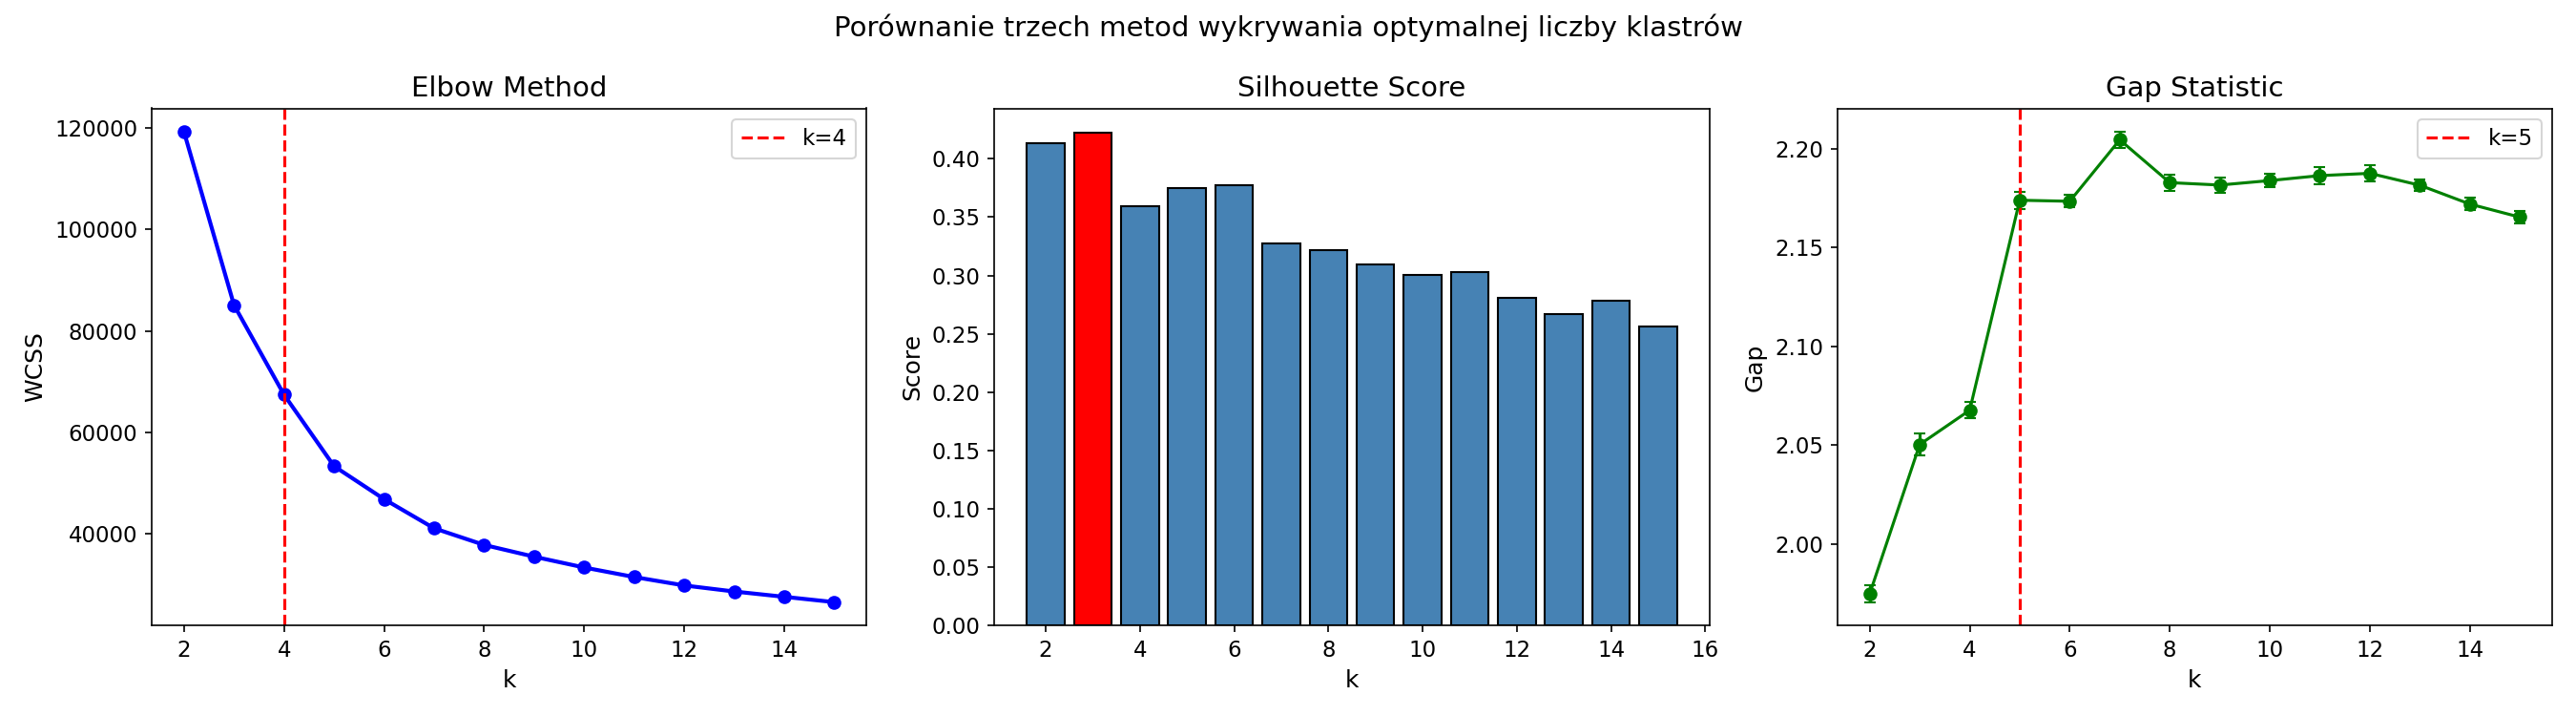
\includegraphics[width=\textwidth]{summary_comparison.png}
    \caption{Porównanie trzech metod na jednym wykresie zbiorczym}
\end{figure}

\begin{figure}[H]
    \centering
    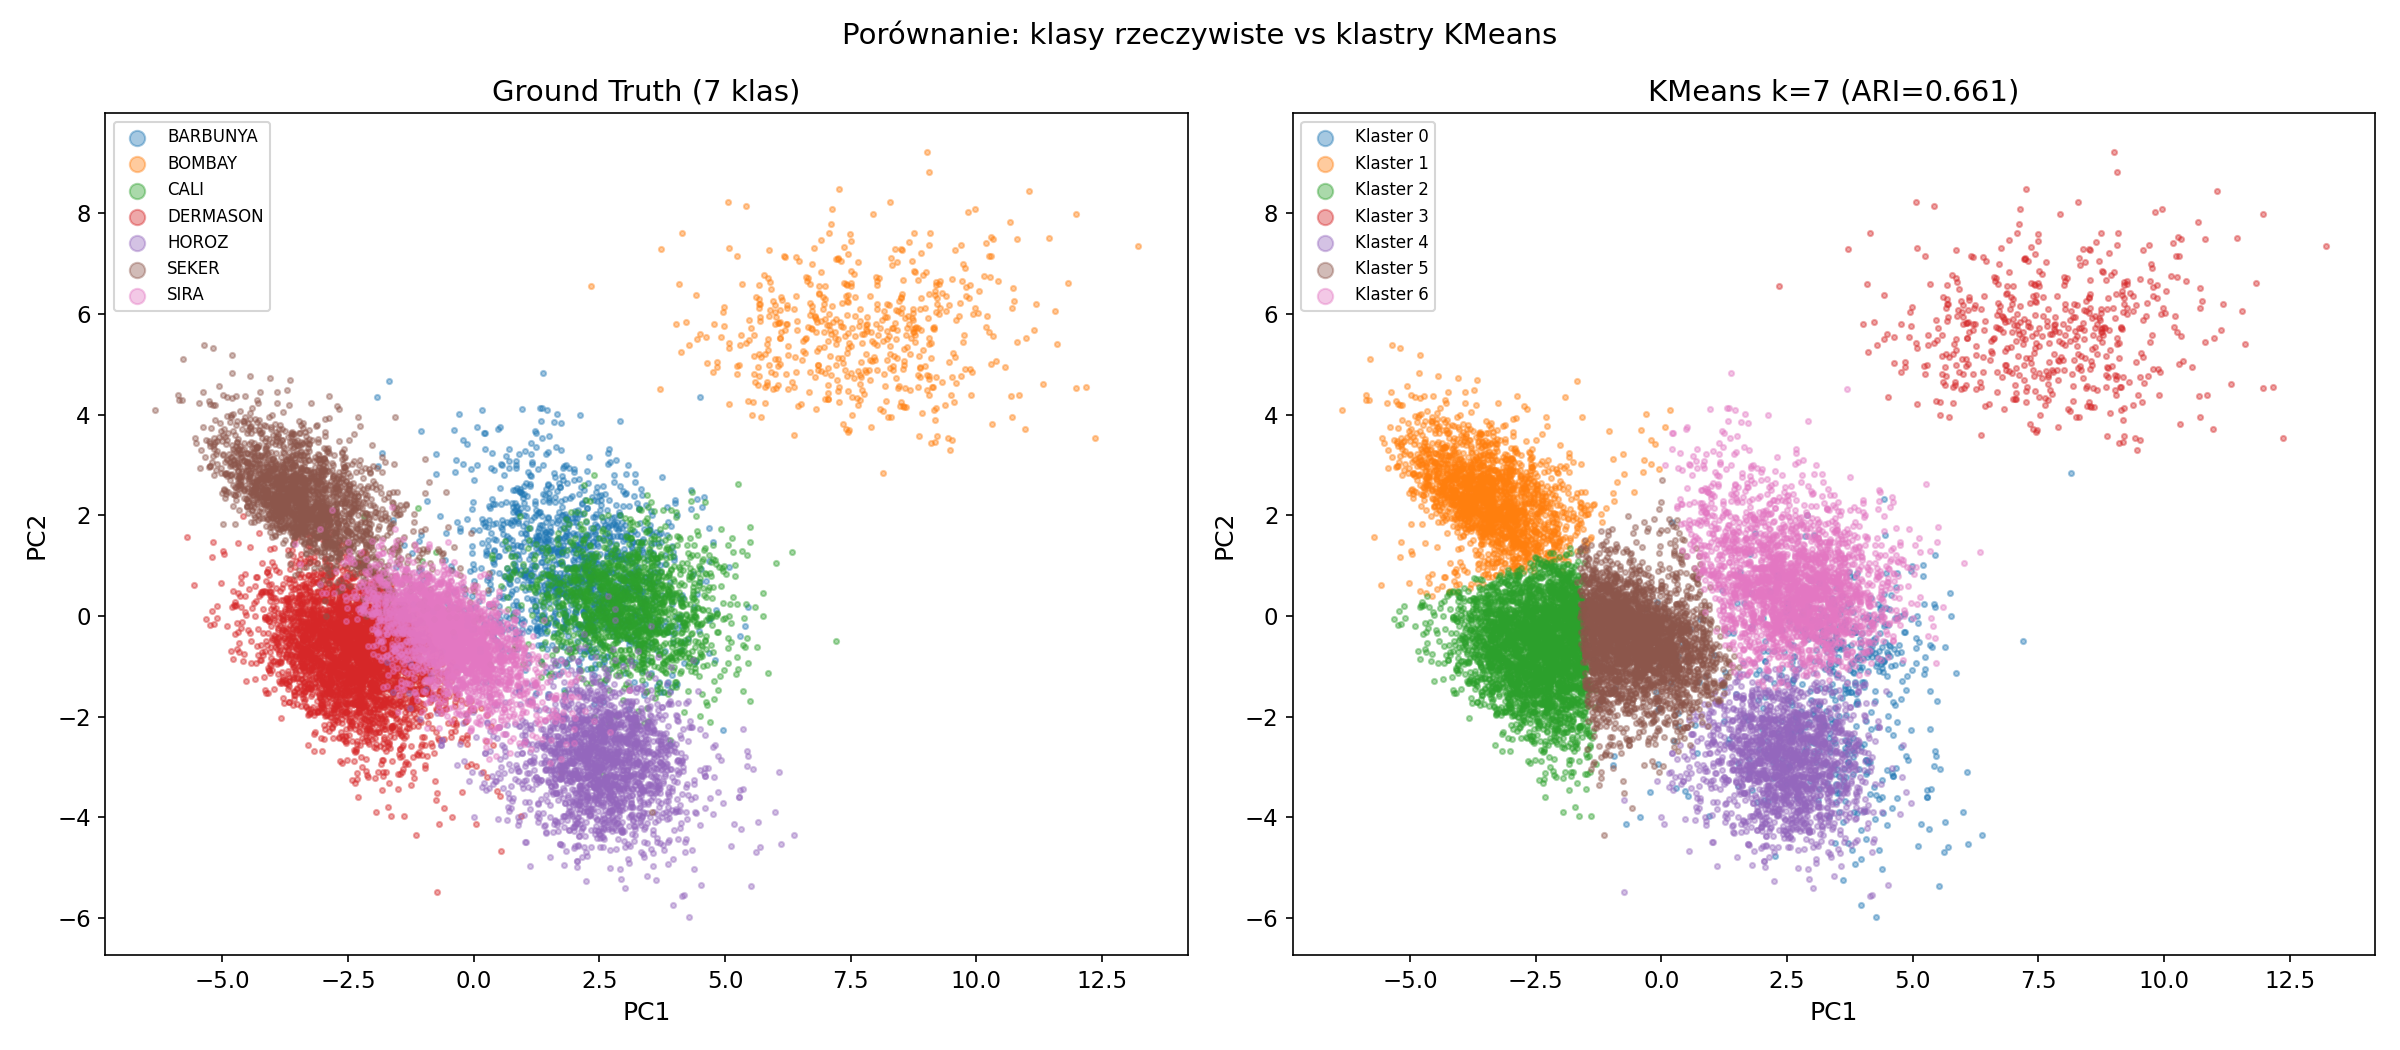
\includegraphics[width=\textwidth]{clusters_vs_ground_truth.png}
    \caption{Wizualna porównanie klastrów dla idealnego scenariusza (KMeans $k=7$) vs Ground Truth}
\end{figure}

\section{Dyskusja}

Przeprowadzone eksperymenty ujawniają ograniczenia standardowych heurystyk klasteryzacyjnych na zbiorach o silnie zachodzących na siebie skupieniach:
\begin{itemize}[leftmargin=1.5cm]
    \item \textbf{Która metoda osiągnęła najlepsze wyniki?} Gap Statistic ($k=5$) okazała się najdokładniejsza. Osiągnięte przy tym wyniki ARI (0.547) i NMI (0.680) stanowiły najlepsze przybliżenie struktury danych.
    \item \textbf{Dlaczego Silhouette Score zaniżył $k$?} Metoda sylwetki dąży do optymalizacji separacji międzygrupowej oraz minimalizacji odległości wewnątrzgrupowych. W zbiorach naturalnie wypukłych i blisko ułożonych klas, metoda ta ma tendencję do łączenia bliskich klas w większe konglomeraty, stąd wskazanie $k=3$.
    \item \textbf{Ograniczenia analizy:} Głównym wyzwaniem jest znaczne nakładanie się cech dla klas takich jak Seker, Dermason i Sira, co powoduje, że nawet algorytm posiadający wiedzę o właściwej liczbie klas ($k=7$) nie osiąga perfekcyjnego dopasowania (ARI na poziomie zaledwie 0.66).
\end{itemize}
Standaryzacja i PCA znacząco ułatwiły procedurę modelowania, pomimo wysokiej redukcji wymiarowości zachowano aż 95\% wariancji.

\section{Wnioski}

Główne wnioski z przeprowadzonego projektu badawczego to:
\begin{itemize}[leftmargin=1.5cm]
    \item Gap Statistic okazała się metodą najmniej podatną na sztuczne łączenie nakładających się klastrów i dała odpowiedź najbliższą wartościom rzeczywistym ($k=5$).
    \item Elbow Method znalazła sensowny kompromis ($k=4$), jednak polega na subiektywnej ocenie punktu przegięcia.
    \item Żadna heurystyka nie rozpoznała poprawnie wszystkich 7 klas. Zastosowanie samych metod opartych na centroidach i odległościach metrycznych może prowadzić do mylnych wniosków biznesowych w przypadku płynnych granic między klasami.
    \item W praktyce eksploracji danych należy stosować metody te jako uzupełniające i polegać dodatkowo na wiedzy dziedzinowej eksperta.
\end{itemize}

\section*{Oświadczenie o reprodukowalności}

Wszystkie eksperymenty przeprowadzono w sposób automatyczny i powtarzalny. W dołączonym repozytorium znajduje się:
\begin{itemize}[leftmargin=1.5cm]
    \item Kod źródłowy w języku Python (\texttt{main.py}),
    \item Informacje o wersjach bibliotek: Python 3.10, pandas 2.2, numpy 1.26, scikit-learn 1.5,
    \item Zbiór danych: \textit{Dry Bean Dataset}.
\end{itemize}
Uruchomienie skryptu generuje reprodukowalne pliki CSV z wynikami ewaluacji oraz zestaw grafik zastosowanych w tym raporcie.

\begin{thebibliography}{99}

\bibitem{koklu}
M. Koklu, I.A. Ozkan,
\textit{Multiclass Classification of Dry Beans Using Computer Vision and Machine Learning Techniques},
Computers and Electronics in Agriculture, 174, 105507, 2020.

\bibitem{tibshirani}
R. Tibshirani, G. Walther, T. Hastie,
\textit{Estimating the number of clusters in a data set via the gap statistic},
Journal of the Royal Statistical Society, B, 63(2), 411--423, 2001.

\bibitem{rousseeuw}
P.J. Rousseeuw,
\textit{Silhouettes: a graphical aid to the interpretation and validation of cluster analysis},
Journal of Computational and Applied Mathematics, 20, 53--65, 1987.

\end{thebibliography}

\end{document}
